\documentclass[11pt,letterpaper]{article}
\usepackage[spanish,es-noshorthands,es-tabla]{babel}
\usepackage{fontspec}
\setmainfont{texgyretermes}[Extension=.otf,UprightFont=*-regular,BoldFont=*-bold,ItalicFont=*-italic,BoldItalicFont=*-bolditalic]
\usepackage[margin=2.5cm]{geometry}
\usepackage{setspace}
\setstretch{1.15}
\usepackage{graphicx}
\usepackage{float}
\usepackage{booktabs}
\usepackage{tabularx}
\usepackage{array}
\usepackage{enumitem}
\setlist{nosep,leftmargin=1.4em}
\usepackage[font=small,labelfont=bf]{caption}
\captionsetup[table]{position=top}
\usepackage{titlesec}
\titleformat{\section}{\large\bfseries}{\thesection.}{0.5em}{}
\titleformat{\subsection}{\normalsize\bfseries}{\thesubsection.}{0.5em}{}
\titlespacing*{\section}{0pt}{1.1em}{0.5em}
\titlespacing*{\subsection}{0pt}{0.8em}{0.3em}
\setlength{\parskip}{0.45em}
\setlength{\parindent}{0pt}
\setlength{\emergencystretch}{3em}
\usepackage{xcolor}
\usepackage[hidelinks]{hyperref}
\hypersetup{colorlinks=true,urlcolor=blue!55!black,linkcolor=black,citecolor=black}
\usepackage{xurl}
\urlstyle{same}
\newcolumntype{Y}{>{\raggedright\arraybackslash}X}
% Citas APA en texto (referencias manuales al final)
\newcommand{\citekey}[2]{\expandafter\def\csname cite@#1\endcsname{#2}}
\citekey{gambetta}{Gambetta, s.~f.}
\citekey{unesco2024}{UNESCO, 2024}
\citekey{onu2015}{Naciones Unidas, 2015}
\citekey{dropgrow}{Shane Staller Games, 2026}
\citekey{kleppmann}{Kleppmann, 2017}
\citekey{lamport}{Lamport, 1978}
\citekey{azurepatterns}{Microsoft, s.~f.-a}
\citekey{azurecicd}{Microsoft, s.~f.-b}
\citekey{nygard}{Nygard, 2018}
\citekey{hudson}{Hudson, 2018}
\citekey{grpc}{gRPC Authors, s.~f.}
\citekey{openapi}{OpenAPI Initiative, 2021}
\citekey{driessen}{Driessen, 2010}
\newcommand{\parencite}[1]{(\csname cite@#1\endcsname)}
\newcommand{\repo}{https://github.com/iadev2005/hydrovalley}
\newcommand{\site}{https://iadev2005.github.io/hydrovalley}
\newcommand{\diag}[2]{#2\footnote{\url{\site/diagrams/#1}}}

\begin{document}

% ---------------------------------------------------------------- Portada
\begin{titlepage}
\centering

\includegraphics[width=0.72\textwidth]{logo/ucab-logo.png}\par
\vspace{1.4cm}
{\large Universidad Católica Andrés Bello – Extensión Guayana\par
\vspace{0.3em}Facultad de Ingeniería\par
\vspace{0.6em}Escuela de Ingeniería Informática\par
\vspace{0.6em}Cátedra: Sistemas Distribuidos y Computación en la Nube\par
\vspace{0.6em}Puerto Ordaz – Estado Bolívar\par}
\vspace{3.2cm}
{\LARGE\bfseries HydroValley: sistema distribuido nativo en la nube para un juego incremental multijugador sobre las 3R del agua\par}
\vspace{3.4cm}
\begin{minipage}[t]{0.45\textwidth}
\raggedright\large
\textbf{Docente:}\par\vspace{0.5em}
Lárez, Jesús
\end{minipage}\hfill
\begin{minipage}[t]{0.45\textwidth}
\raggedleft\large
\textbf{Estudiantes:}\par\vspace{0.5em}
Aliendres, Ignacio\par
Baczek, Cristian\par
Palma, Alfonso\par
Pérez, Fernando
\end{minipage}
\vfill
{\large Ciudad Guayana, 30 de octubre de 2026\par}
\end{titlepage}

\setcounter{page}{2}

% ---------------------------------------------------------------- 1
\section{Introducción}

Los sistemas que atienden a muchos usuarios a la vez sobre un estado compartido enfrentan los problemas clásicos de la computación distribuida: concurrencia, ausencia de memoria y de reloj comunes, fallos parciales y la necesidad de que los contadores cuadren aunque una máquina se apague. Los videojuegos en línea son un caso extremo de ese escenario, porque cada acción debe responder al instante y el resultado tiene que ser idéntico para todos los jugadores \parencite{gambetta}.

En este trabajo se desarrolló \textit{HydroValley}, un juego incremental cooperativo sobre el cuidado del agua. Los jugadores sueltan gotas sobre un valle isométrico de $32 \times 32$ casillas, compartido por todos y simulado en el servidor; con las hojas que obtienen compran instalaciones de las 3R (reducir, reutilizar y reciclar) que riegan solas. Por dentro, el juego es un conjunto de cinco servicios propios escritos en cuatro lenguajes (TypeScript, Go, Rust y Python), más PostgreSQL, que se comunican por gRPC y se despliegan en contenedores repartidos entre las máquinas del laboratorio.

El informe se organiza en siete secciones. En la sección 2 se plantean el problema, su relación con los Objetivos de Desarrollo Sostenible y los objetivos del proyecto; la sección 3 analiza el problema y deriva los requerimientos; la sección 4 presenta el diseño de la solución y los patrones de la nube aplicados; la sección 5 describe la implementación, la documentación de la API y el pipeline de CI/CD; la sección 6 reporta las pruebas ejecutadas con sus cifras, y la sección 7 recoge las conclusiones. Los recursos del proyecto pueden consultarse en línea (ver Tabla~\ref{tab:recursos}).

\begin{table}[H]
\centering\small
\caption{Recursos del proyecto}
\label{tab:recursos}
\begin{tabularx}{\textwidth}{@{}lY@{}}
\toprule
Recurso & Dirección \\
\midrule
Documentación de la API (Swagger) & \url{https://iadev2005.github.io/hydrovalley/api.html} \\
Página del proyecto y diagramas & \url{https://iadev2005.github.io/hydrovalley/} \\
Código fuente & \url{https://github.com/iadev2005/hydrovalley} \\
\bottomrule
\end{tabularx}
\end{table}

% ---------------------------------------------------------------- 2
\section{El problema y la propuesta}

\subsection{Planteamiento del problema}

Para 2022, unos 2.200 millones de personas carecían de agua potable gestionada de forma segura \parencite{unesco2024}. La Agenda 2030 recoge esa urgencia en el Objetivo 6, que incluye aumentar el uso eficiente de los recursos hídricos, y en el Objetivo 12, que pide reducir los desechos mediante la prevención, la reducción, el reciclado y la reutilización \parencite{onu2015}. Las 3R son, por tanto, un tema con peso social, pero difícil de transmitir con mensajes abstractos: la eficiencia hídrica se entiende mejor cuando se ve su efecto acumulado en el tiempo.

El curso, por su parte, exigía construir un sistema distribuido con al menos cuatro lenguajes, comunicación gRPC, contenedores, un pipeline de CI/CD, documentación Swagger y despliegue en el laboratorio. El reto consistió en encontrar un dominio en el que esos requisitos no fueran decoración, sino respuesta a problemas reales del propio sistema.

\subsection{Propuesta}

Se propuso un juego del género \textit{clicker} incremental, inspirado en la mecánica de \textit{Drop and Grow} \parencite{dropgrow}, pero con un valle único, permanente y compartido. Cada gota cuesta 1 L del depósito del jugador; con suficiente humedad la casilla sube de etapa (tierra seca, pasto, arbusto, flores y árbol) y quien la hizo crecer gana hojas. Con las hojas se compran tres instalaciones, una por cada R: el aspersor de agua gris (reutilizar), el riego por goteo, que reduce la evaporación a la mitad (reducir), y la planta de tratamiento, que recarga el depósito más rápido (reciclar). El valle se evapora, se marchita y arde al azar, de modo que el ahorro de agua es una necesidad dentro del juego y no un mensaje externo.

La decisión de diseño que guió el proyecto fue que \textbf{el agua es el tema y la concurrencia es el examen}. La mecánica de \textit{farmeo} produce exactamente los problemas que evalúa la materia (ver Tabla~\ref{tab:farmeo}).

\begin{table}[H]
\centering\small
\caption{Problemas distribuidos que provoca la mecánica del juego}
\label{tab:farmeo}
\begin{tabularx}{\textwidth}{@{}lY@{}}
\toprule
Lo que provoca el farmeo & Problema distribuido que plantea \\
\midrule
Muchas acciones pequeñas a la vez & Concurrencia sobre un estado compartido \\
Cada acción debe responder al instante & Baja latencia entre servicios (de ahí gRPC) \\
Los contadores de agua y hojas deben cuadrar & Consistencia: ni pérdidas ni duplicados \\
El estado vive repartido entre máquinas & Sin memoria ni reloj compartidos; fallos parciales \\
\bottomrule
\end{tabularx}
\end{table}

\subsection{Relación con los Objetivos de Desarrollo Sostenible}

El proyecto se vincula con tres ODS \parencite{onu2015}:
\begin{itemize}
\item \textbf{ODS 6, Agua limpia y saneamiento (meta 6.4).} La mecánica central premia el uso eficiente del agua: el depósito es limitado, la humedad se evapora y el riego por goteo reduce esa pérdida a la mitad.
\item \textbf{ODS 12, Producción y consumo responsables (meta 12.5).} Las tres instalaciones modelan la reducción, la reutilización del agua gris y el reciclaje en una planta de tratamiento. El reporte de las 3R muestra al jugador cuánta agua ahorró, reutilizó y recicló.
\item \textbf{ODS 4, Educación de calidad (meta 4.7).} El juego es un recurso lúdico para aprender sobre desarrollo sostenible: el jugador comprueba por sí mismo que, sin instalaciones, el valle se seca más rápido de lo que puede regarlo a mano.
\end{itemize}

\subsection{Objetivos}

\textbf{Objetivo general.} Desarrollar un sistema distribuido nativo en la nube para un juego incremental multijugador sobre las 3R del agua.

\textbf{Objetivos específicos.}
\begin{enumerate}
\item Analizar los requisitos del proyecto y las alternativas de juego, de modelo de ejecución y de tecnología.
\item Definir los requerimientos funcionales y no funcionales con base en el análisis realizado.
\item Diseñar la arquitectura de servicios y sus contratos gRPC según los requerimientos definidos.
\item Construir los servicios, los contenedores y el pipeline de CI/CD con base en el diseño elaborado.
\item Validar el sistema mediante pruebas de carga, de consistencia y de tolerancia a fallos.
\end{enumerate}

\subsection{Alcance y limitaciones}

El alcance se dividió en dos niveles. El \textbf{nivel 1}, obligatorio, comprendió el valle con gotas, humedad, crecimiento, evaporación y marchitamiento, las tres instalaciones, dos mejoras, los incendios, el límite de gotas, el ranking, las instantáneas con recuperación, el proxy, los bots, el panel del sistema y el pipeline. Del \textbf{nivel 2} se completaron el despliegue repartido en el laboratorio, el chat, la propagación del fuego, la comparativa Go vs.\ Rust, el resumen al volver y y el monitoreo con Prometheus y Grafana. No se contempló enviar a cada jugador solo su parte del mundo, ni usar Kubernetes o \textit{streams} de gRPC.

Las limitaciones principales fueron del laboratorio: equipos con Windows 10 y Docker Desktop sobre WSL~2, una cuenta sin permisos de administrador y un cortafuegos que bloqueaba las conexiones entre máquinas. Para mitigarlas, el sistema se desarrolló primero en una sola máquina (plan B) y se diseñó para pasar al despliegue repartido (plan A) cambiando solo configuración; el encargado del laboratorio abrió los puertos necesarios desde la subred.

% ---------------------------------------------------------------- 3
\section{Análisis del problema}

\subsection{Alternativas evaluadas}

Teniendo el problema delimitado, se compararon cuatro tipos de juego: un \textit{clicker} cooperativo, un \textit{tycoon}, un juego por turnos y uno de cooperación en tiempo real al estilo de \textit{Overcooked}. Se eligió el \textit{clicker} porque los bots que lo simulan son triviales, porque su estado se verifica con un número (las cuentas deben cuadrar) y porque su riesgo de no terminar a tiempo era el menor. El juego en tiempo real se descartó porque convierte el proyecto en un problema de \textit{netcode} y de predicción en el cliente, que no es lo que se evalúa \parencite{gambetta}.

En cuanto al modelo de ejecución, se descartaron la aplicación tradicional, que no comparte estado, y la transmisión de video del juego. Se adoptó un \textbf{servidor autoritativo}, como en los juegos multijugador masivos: el servidor es el único que calcula el mundo y el navegador solo dibuja y envía intenciones.

\subsection{Requerimientos}

Con base en el análisis anterior se definieron 31 requerimientos funcionales, 12 no funcionales y 7 restricciones. La Tabla~\ref{tab:req} resume los más relevantes; cada no funcional se redactó con una cifra para poder verificarlo en las pruebas. El equipo declaró que cuatro elementos nunca se recortarían: RF-08, RF-09, RF-21 y RES-01.

\begin{table}[H]
\centering\small
\caption{Requerimientos principales}
\label{tab:req}
\begin{tabularx}{\textwidth}{@{}lY@{}}
\toprule
ID & Requerimiento \\
\midrule
RF-05 & El sistema debe rechazar más de 15 gotas por segundo de un mismo jugador. \\
RF-08 & El sistema debe procesar acciones simultáneas del mismo jugador sin duplicar ni perder recursos. \\
RF-09 & El sistema debe aplicar una sola vez una acción repetida con el mismo identificador. \\
RF-10 / RF-11 & El sistema debe calcular el ranking global por hojas ganadas sin pausar el juego. \\
RF-14 & El chat debe mostrar los mensajes en el mismo orden a todos los jugadores. \\
RF-23 / RF-24 & El mundo debe recuperarse desde la última instantánea y sobrevivir al reinicio del hub. \\
RF-21 / RF-22 & El pipeline debe compilar, probar y empaquetar, y rechazar código que rompa las pruebas. \\
RF-29 & Los incendios deben depender de un azar con semilla, reproducible. \\
RNF-01 & El sistema debe sostener al menos 100 acciones/s con 30 bots. \\
RNF-02 & El 95 \% de las acciones debe resolverse en menos de 200 ms. \\
RNF-04 & Si cae un servicio secundario, las gotas deben seguir respondiendo en menos de 200 ms. \\
RNF-05 & Ningún evento se ordena por el reloj de una máquina; el orden lo da el tick. \\
RNF-09 & Los servicios deben arrancar en cualquier orden y reconectarse solos. \\
RNF-10 & El sistema debe levantarse desde cero en menos de 5 minutos. \\
\midrule
RES-01 & Toda comunicación interna usa gRPC. \\
RES-02 & Go y Rust son obligatorios, más TypeScript y Python. \\
RES-03 / RES-06 & Un contenedor por servicio y un pipeline de CI/CD. \\
RES-04 / RES-05 & API documentada con Swagger/OpenAPI y diseño en UML. \\
RES-07 & Despliegue repartido en las máquinas del laboratorio. \\
\bottomrule
\end{tabularx}
\end{table}

Los casos de uso que originan estos requerimientos están en el \diag{casos-de-uso.svg}{diagrama de casos de uso}, con tres actores: jugador, bot y administrador.

% ---------------------------------------------------------------- 4
\section{Diseño de la solución}

\subsection{Arquitectura de servicios}

Teniendo los requerimientos definidos, se diseñó una arquitectura de seis piezas, cada una en su contenedor (ver Figura~\ref{fig:componentes}). El proxy nginx es la única puerta de entrada: enruta \texttt{/api} a la API, \texttt{/play} al hub y \texttt{/chat} al chat. La \textbf{API} (TypeScript) atiende el registro, el acceso con token firmado, el catálogo, el ranking y los reportes. El \textbf{hub} (Go) mantiene una goroutine por jugador conectado por WebSocket, filtra las acciones y marca el tick cada 100 ms. El \textbf{simulador} (Rust) es el único que modifica el mundo. La \textbf{persistencia} (Python) es la única con credenciales de PostgreSQL. El \textbf{chat} (Go) ordena los mensajes con un número de secuencia.

\begin{figure}[H]
\centering
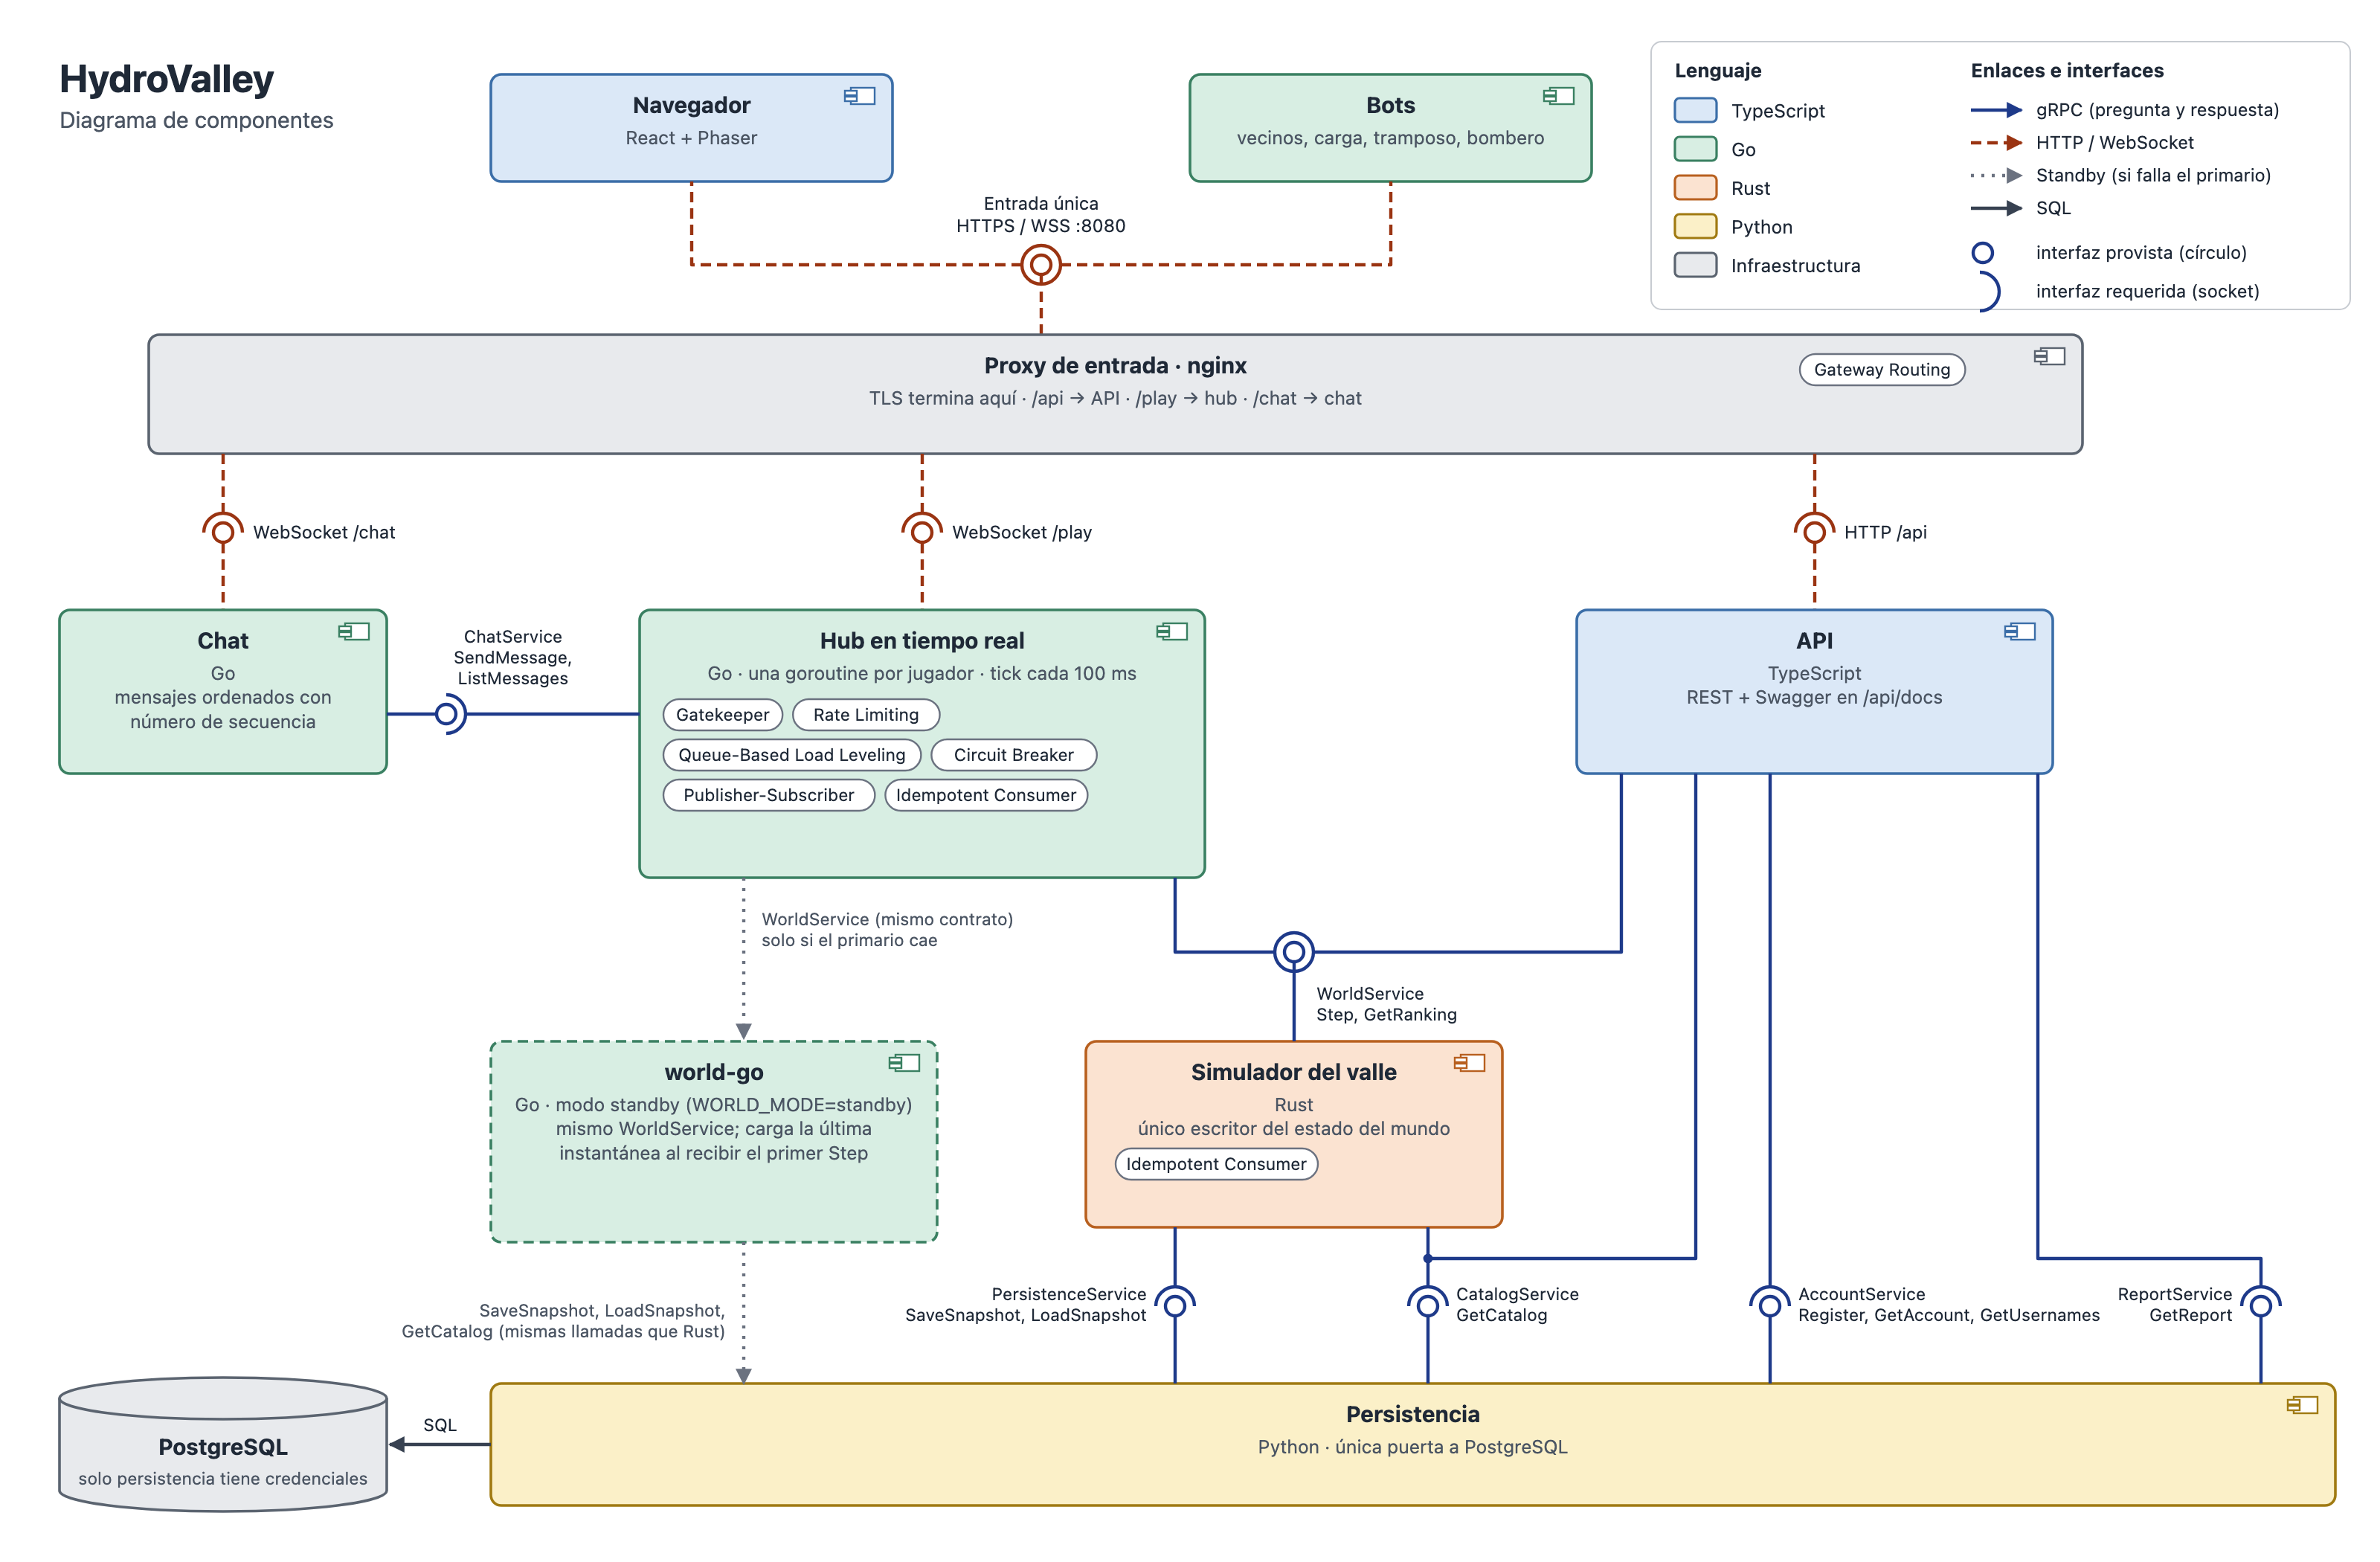
\includegraphics[width=\textwidth]{fig/componentes.png}
\caption{Diagrama de componentes en notación lollipop. Versión ampliada en \url{\site/diagrams/componentes.svg}.}
\label{fig:componentes}
\end{figure}

En la figura se aprecia que ningún servicio llama directamente a la base de datos salvo la persistencia, y que cada interfaz gRPC tiene un único proveedor. La frontera más importante es la de Go y Rust: \textbf{Go decide si un comando es admisible; Rust decide qué produce}. El hub valida la sesión, el rol, el identificador de la acción y el límite de gotas, pero nunca calcula el mundo; el simulador calcula crecimiento, saldos, fuego y ranking, pero nunca toca una conexión de jugador.

\subsection{Consistencia sin reloj compartido}

Para cumplir RF-08 y RF-09 se diseñaron cinco capas complementarias:
\begin{enumerate}
\item \textbf{Filtro por jugador.} Cada conexión tiene su goroutine, que aplica las reglas de admisión antes de encolar.
\item \textbf{Escritor único.} Solo el simulador modifica el estado, en un solo hilo y una vez por tick. La carrera clásica de leer 100 y escribir 110 desde dos máquinas es imposible por construcción \parencite{kleppmann}.
\item \textbf{Idempotencia.} Toda acción lleva un \texttt{action\_id} (UUID). El hub recuerda las acciones pendientes y las confirmadas durante 60 s, y el simulador recuerda las aplicadas en los últimos 600 ticks dentro de la instantánea. Cada acción admitida recibe exactamente un resultado final: \texttt{applied}, \texttt{duplicate}, \texttt{rejected} o \texttt{expired}.
\item \textbf{Tick como reloj lógico.} Los eventos se ordenan por el número de tick, nunca comparando relojes de máquinas distintas \parencite{lamport}.
\item \textbf{Instantáneas.} Cada 50 ticks (5 s) el simulador envía una copia del mundo a la persistencia desde una tarea en segundo plano. Si ya existe una fila para ese tick, la persistencia compara época y huella SHA-256 para distinguir un reintento de un conflicto.
\end{enumerate}

El azar también es determinista: solo el simulador lo decide, con un generador con semilla cuyo estado viaja en la instantánea, de modo que la misma semilla y los mismos comandos producen el mismo valle. Agua, hojas y humedad son enteros de 64 bits sin signo, nunca decimales. El flujo completo de una gota se muestra en el \diag{secuencia-gota.svg}{diagrama de secuencia de la gota}, y los estados de una casilla en el \diag{estados-casilla.svg}{diagrama de estados}.

\subsection{Patrones de diseño en la nube}

Se aplicaron nueve patrones del catálogo de Microsoft \parencite{azurepatterns}. Para cada uno se documentó qué problema resuelve, dónde está en el código y qué ocurriría sin él (ver Tabla~\ref{tab:patrones}).

\begin{table}[H]
\centering\small
\caption{Patrones de diseño en la nube aplicados}
\label{tab:patrones}
\begin{tabularx}{\textwidth}{@{}lp{3.2cm}Y@{}}
\toprule
Patrón & Dónde & Uso concreto \\
\midrule
Circuit Breaker & Hub & Tras 3 fallos seguidos de \texttt{Step} deja de llamar al simulador, avisa a los jugadores y prueba cada 1 s \parencite{nygard}. \\
Gatekeeper & Hub & Valida sesión, rol, duplicado y cuota antes de que la acción llegue al simulador. \\
Rate Limiting & Hub y API & 15 gotas/s por jugador; límites por IP y por usuario en registro y acceso. \\
Queue-Based Load Leveling & Hub & Cola de hasta 5.000 comandos, lotes de 500 por tick, caducidad a los 30 s. \\
Publisher-Subscriber & Hub y chat & Difunde el estado una vez por segundo; expulsa al consumidor lento. \\
Health Endpoint Monitoring & Todos & \texttt{/healthz}, \texttt{/readyz} y \texttt{grpc.health.v1}; el panel \texttt{/sistema.html} los agrega. \\
Retry con espera exponencial & Simulador y API & 100, 200 y 400 ms, solo en llamadas idempotentes. \\
Gateway Routing & nginx & Única entrada HTTPS en el 8080; añade \texttt{X-Request-Id} de punta a punta. \\
Idempotent Consumer & Hub y simulador & El \texttt{action\_id} evita aplicar dos veces la misma acción. \\
\bottomrule
\end{tabularx}
\end{table}

\subsection{Despliegue y alta disponibilidad}

El sistema se diseñó para dos topologías con las mismas imágenes. En el \textbf{plan B} todo corre en una máquina con Docker Compose; en el \textbf{plan A} cada máquina del laboratorio levanta su propio archivo Compose (base de datos, persistencia, simulador, hub con chat y proxy con la API). Pasar de uno a otro es solo configuración: ninguna dirección está en el código y cada servicio lee de variables de entorno a quién llama. Se descartaron Kubernetes y Docker Swarm porque el NAT de WSL~2 y los puertos cerrados los hacían frágiles en el laboratorio. La topología real se muestra en el \diag{despliegue.svg}{diagrama de despliegue}.

Para tolerar la caída de una máquina se añadió un nodo de respaldo con \texttt{world-go}, una versión en Go del simulador. El respaldo arranca en modo \textit{standby} y solo carga la última instantánea cuando recibe el primer paso. Para que nunca escriban dos simuladores a la vez, cada llamada \texttt{Step} lleva la generación del hub: el simulador rechaza con \texttt{FAILED\_PRECONDITION} a cualquier hub de generación menor, que queda retirado. Además, si un simulador despierta con un tick menor al esperado, invalida su memoria y recarga la instantánea, de modo que el tick nunca retrocede. El objetivo fijado fue recuperarse en 10 s como máximo, perdiendo a lo sumo 50 ticks (5 s). El relevo se ilustra en la \diag{reinicio-simulador.svg}{secuencia de reinicio del simulador}.

% ---------------------------------------------------------------- 5
\section{Implementación}

\subsection{Tecnologías}

Habiendo definido la arquitectura, se procedió a construir cada servicio con la estructura oficial de su lenguaje. La Tabla~\ref{tab:tec} muestra las versiones usadas. Rust se reservó para el simulador porque su papel exige un escritor único, determinista y sin pausas; no se argumentó por el recolector de basura de Go, cuyas pausas están por debajo del milisegundo \parencite{hudson}, frente a un tick de 100 ms.

\begin{table}[H]
\centering\small
\caption{Tecnologías y versiones}
\label{tab:tec}
\begin{tabularx}{\textwidth}{@{}llY@{}}
\toprule
Servicio & Lenguaje y versión & Bibliotecas principales \\
\midrule
API & TypeScript 6.0 sobre Node 22 & Fastify 5.12, \texttt{@fastify/swagger} 9.9, Connect 2.2, Argon2 \\
Frontend & TypeScript, React 19 & Phaser 4 para el valle isométrico, Vite 8 \\
Hub, chat y bots & Go 1.26 & \texttt{coder/websocket} 1.8, verificación de tokens Ed25519 \\
Simulador & Rust 1.97 (edición 2024) & tonic 0.14, prost 0.14, tokio 1.53 \\
Simulador de respaldo & Go 1.26 & Puerto fiel del simulador de Rust \\
Persistencia & Python 3.12 & \texttt{grpcio} 1.76, \texttt{psycopg} 3.2 \\
Base de datos y proxy & PostgreSQL 16, nginx 1.30 & Imagen sin privilegios; TLS en el 8080 \\
\bottomrule
\end{tabularx}
\end{table}

\subsection{Contratos gRPC y API REST}

Los contratos se escribieron antes que el código, en archivos \texttt{.proto} bajo el paquete \texttt{hydrovalley.<servicio>.v1} \parencite{grpc}. Se definieron \texttt{WorldService} (\texttt{Step}, \texttt{GetRanking}), \texttt{PersistenceService} (\texttt{SaveSnapshot}, \texttt{LoadSnapshot}), \texttt{AccountService}, \texttt{CatalogService}, \texttt{ReportService} y \texttt{ChatService}. No se usaron \textit{streams}: todas las llamadas son de pregunta y respuesta con plazo, y solo las idempotentes se reintentan. La herramienta \texttt{buf} valida el estilo y detecta cambios incompatibles en cada pull request.
{\sloppy \par}
La API REST se documentó con OpenAPI 3.1 \parencite{openapi}. La interfaz de Swagger se sirve en \texttt{/api/docs} de cada despliegue. \textbf{La documentación completa de la API puede consultarse en \url{\site/api.html}}, con cada ruta, sus parámetros, sus respuestas y sus códigos de error. La especificación describe el registro, el acceso, el catálogo, el ranking, los reportes y el estado del sistema. Las contraseñas se guardan con Argon2id, el token se firma con Ed25519 y dura 12 h, y TLS termina en nginx.

\subsection{Integración y entrega continuas}

El pipeline de GitHub Actions tiene un trabajo por servicio, activado solo cuando cambian sus archivos \parencite{azurecicd}. Cada trabajo comprueba el formato, ejecuta el análisis estático (\texttt{clippy}, \texttt{go vet}, \texttt{staticcheck}, ESLint, \texttt{tsc} estricto) y corre las pruebas unitarias; las de Go usan el detector de carreras. En cada pull request un trabajo adicional construye todas las imágenes para \texttt{linux/amd64}, levanta el sistema completo y ejecuta las pruebas de punta a punta, incluidas las de fallos. Al fusionar en \texttt{dev}, las imágenes se publican en \texttt{ghcr.io} con la etiqueta \texttt{dev}; al etiquetar \texttt{main}, con la versión. Las ramas \texttt{main} y \texttt{dev} exigen pull request y CI en verde, y bloquean el \textit{force push} \parencite{driessen}.

\subsection{Despliegue en el laboratorio}

El 23 de octubre de 2026 el sistema se desplegó en cinco equipos del laboratorio, uno por nodo, con un script de PowerShell que levanta cada nodo a partir de las direcciones y los secretos de esa máquina. La Tabla~\ref{tab:lab} resume las incidencias encontradas y cómo se resolvieron.

\begin{table}[H]
\centering\small
\caption{Incidencias del despliegue en el laboratorio}
\label{tab:lab}
\begin{tabularx}{\textwidth}{@{}YY@{}}
\toprule
Incidencia & Solución \\
\midrule
El cortafuegos bloqueaba los puertos entre máquinas & El encargado creó una regla de entrada para 8080, 8081, 8082, 50051 y 5433 desde la subred \\
\texttt{unauthorized} al descargar imágenes de \texttt{ghcr.io} & Inicio de sesión con un token de solo lectura de paquetes \\
El diagnóstico no distinguía un puerto bloqueado de uno sin servicio & Se añadió un modo que abre un puerto de prueba antes de levantar el nodo \\
Los puertos 80 y 5432 estaban ocupados por el laboratorio & El proxy se publicó en el 8080 y PostgreSQL en el 5433 \\
\bottomrule
\end{tabularx}
\end{table}

% ---------------------------------------------------------------- 6
\section{Pruebas – Ejecución}

\subsection{Casos de prueba}

Una vez construido el sistema, se procedió a validarlo con doce casos de prueba, CP-01 a CP-12, cada uno trazado a un requerimiento. Los casos de fallos se automatizaron y corren en el CI tanto deteniendo como pausando contenedores. La Tabla~\ref{tab:cp} reporta los resultados. Salvo CP-11, las cifras se midieron en el plan B (equipo de desarrollo y ejecutor del CI).

\begin{table}[H]
\centering\small
\caption{Resultados de los casos de prueba}
\label{tab:cp}
\begin{tabularx}{\textwidth}{@{}llY@{}}
\toprule
Caso & Req. & Resultado \\
\midrule
CP-01: 100 gotas simultáneas & RF-08 & 100 enviadas, 100 aplicadas; la humedad subió exactamente 100. \\
CP-02: reenvío con el mismo ID & RF-09 & El reenvío recibe \texttt{duplicate} y se aplica una sola vez. \\
CP-03: tramposo a 50 gotas/s & RF-05 & De 501 gotas en 10 s, 150 admitidas (15/s) y 351 \texttt{rate\_limited}. \\
CP-04: 3 bots sobre un incendio & RF-30 & Un solo incendio apagado y un solo bono. \\
CP-05: caída del simulador & RF-23 & Detectada en 1 s y recuperada en 1–3 s, con 9–16 ticks perdidos (límite: 50). Con apagado ordenado o pausa, 0 ticks perdidos. \\
CP-06: caída del hub & RF-24 & Detectada en 1,1–1,3 s; reconexión en 0,1–0,3 s; la acción reenviada se aplicó una vez. \\
CP-07: caída de la persistencia & RNF-04 & Las gotas siguieron con p95 de 68–103 ms; aviso 503 en menos de 1 s. \\
CP-08: arranque en orden inverso & RNF-09 & Todo conectado 7,5 s después del último servicio, sin reinicios. \\
CP-09: orden del chat & RF-14 & Todos los clientes recibieron los mensajes en el mismo orden. \\
CP-10: azar reproducible & RF-29 & Misma semilla y mismos comandos produjeron el mismo valle en Rust y en Go. \\
CP-11: carga con 30 bots & RNF-01/02 & Ver Tabla~\ref{tab:carga}. \\
CP-12: persistencia caída en una instantánea & RF-23 & El tick siguió a 10/s, \texttt{Step} p95 máx.\ 2,4 ms y el \textit{breaker} cerrado. \\
\bottomrule
\end{tabularx}
\end{table}

En CP-05, los ticks perdidos al matar el simulador se explican por diseño: se pierde lo ocurrido desde la última instantánea, que nunca supera 50 ticks. Con un apagado ordenado el simulador guarda una instantánea final, y por eso no se pierde ninguno. El relevo al nodo de respaldo se midió en local con una recuperación de 1,31 s, sin ticks retrocedidos, y la conmutación del \textit{hub} retiró al hub desplazado en 30 ms.

\subsection{Prueba de carga}

La prueba de carga (CP-11) se ejecutó en el laboratorio el 27 de octubre de 2026, con 30 bots durante 60 s lanzados desde el nodo del hub contra las imágenes publicadas (ver Tabla~\ref{tab:carga}).

\begin{table}[H]
\centering\small
\caption{Prueba de carga CP-11 (30 bots, 60 s)}
\label{tab:carga}
\begin{tabular}{@{}lrrrrrr@{}}
\toprule
Entorno & Gotas & Aceptadas & Ritmo (gotas/s) & p50 (ms) & p95 (ms) & Máx.\ (ms) \\
\midrule
Laboratorio (plan A) & 7.178 & 100 \% & 119,6 & 62,4 & 106,5 & 118,9 \\
Equipo de desarrollo (plan B) & 7.156 & — & 119,3 & 53,2 & 99,3 & — \\
\bottomrule
\end{tabular}
\end{table}

En el laboratorio se superaron los dos umbrales: 119,6 acciones/s frente a 100 (RNF-01), y el 100 \% de las acciones por debajo de 200 ms frente al 95 \% exigido (RNF-02). La humedad aportada al valle (7.178) coincidió con las gotas aceptadas, lo que confirma que no hubo pérdidas ni duplicados bajo carga.

\subsection{Comparativa Go vs.\ Rust}

Como el simulador existe en dos lenguajes, se midió el paso del mundo (\texttt{World::step}) en ambos, sin red, con el mismo catálogo y la misma semilla, comprobando que la huella final del valle fuera idéntica. Se tomó la mediana de cuatro ejecuciones en un Apple M4 (ver Tabla~\ref{tab:bench}).

\begin{table}[H]
\centering\small
\caption{Duración mediana de un paso del simulador (µs)}
\label{tab:bench}
\begin{tabular}{@{}lrrr@{}}
\toprule
Tamaño del valle & Rust & Go & Rust / Go \\
\midrule
$32 \times 32$ (juego) & 11,5 & 8,6 & 1,33 \\
$128 \times 128$ & 248,8 & 196,7 & 1,26 \\
$512 \times 512$ & 6.331,4 & 4.589,6 & 1,38 \\
\bottomrule
\end{tabular}
\end{table}

Contra lo esperado, Rust tardó entre un 26 \% y un 38 \% más que Go en todos los tamaños, e incluso con optimizaciones agresivas de enlace Rust no lo alcanzó. El resultado no invalida el diseño: en el valle del juego, un paso tarda unos 10 µs, es decir, la diezmilésima parte de un tick de 100 ms, por lo que cualquiera de los dos sirve y la elección de Rust queda justificada por el reparto de papeles y no por el rendimiento. La medición se realizó en un procesador ARM; en los equipos x86 del laboratorio las cifras absolutas pueden variar, pero la holgura frente al tick es de cuatro órdenes de magnitud.

% ---------------------------------------------------------------- 7
\section{Conclusiones}

Una vez construido el sistema y ejecutadas las pruebas, se concluye que:
\begin{enumerate}
\item Elegir un juego incremental sobre las 3R permitió que cada requisito técnico respondiera a un problema real del propio juego, y vinculó el proyecto con los ODS 4, 6 y 12 sin que el tema fuera decoración.
\item El análisis de alternativas llevó a un servidor autoritativo con escritor único, lo que eliminó por construcción las carreras sobre el estado compartido. CP-01 lo confirmó: 100 gotas simultáneas produjeron exactamente 100 de humedad.
\item La combinación de \texttt{action\_id}, tick como reloj lógico e instantáneas con huella garantizó que ninguna acción se aplicara dos veces ni se perdiera, incluso tras caídas del hub o del simulador (CP-02, CP-05 y CP-06).
\item Separar admisión (Go) de cálculo (Rust) y aplicar patrones como \textit{Circuit Breaker}, \textit{Rate Limiting} y \textit{Queue-Based Load Leveling} permitió que el sistema degradara con elegancia: al caer la persistencia, las gotas siguieron respondiendo por debajo de 103 ms.
\item El despliegue repartido en el laboratorio cumplió los objetivos de rendimiento con margen: 119,6 acciones/s y p95 de 106,5 ms, frente a umbrales de 100 acciones/s y 200 ms.
\item Diseñar los contratos gRPC y la portabilidad entre plan B y plan A desde el inicio hizo que llevar el sistema a cinco máquinas fuera solo un cambio de configuración. Los problemas del laboratorio fueron de red y permisos, no de código.
\item Medir antes de afirmar evitó una conclusión equivocada: Go superó a Rust en el paso del simulador, y la medición mostró que ambos están cuatro órdenes de magnitud por debajo del presupuesto del tick.
\item Automatizar las pruebas de fallos en el pipeline permitió detectar regresiones de tolerancia a fallos en cada pull request, y no solo en la demostración final.
\end{enumerate}

Con base en estas conclusiones se recomienda: extender la comparativa Go vs.\ Rust a la arquitectura x86 y a valles de mayor tamaño; enviar a cada jugador solo la región visible del valle para escalar a mapas más grandes; y cifrar el gRPC interno con TLS mutuo si el sistema se despliega fuera de la red cerrada del laboratorio.

% ---------------------------------------------------------------- Referencias
\section*{Referencias bibliográficas}
\begingroup
\small
\setlength{\parindent}{-1.27cm}\setlength{\leftskip}{1.27cm}\setlength{\parskip}{0.35em}

Driessen, V. (2010). \textit{A successful Git branching model}. \url{https://nvie.com/posts/a-successful-git-branching-model/}

Gambetta, G. (s.~f.). \textit{Fast-paced multiplayer (Part I): Client-server game architecture}. \url{https://www.gabrielgambetta.com/client-server-game-architecture.html}

gRPC Authors. (s.~f.). \textit{Introduction to gRPC}. \url{https://grpc.io/docs/what-is-grpc/introduction/}

Hudson, R. (2018, 12 de julio). \textit{Getting to Go: The journey of Go's garbage collector}. The Go Blog. \url{https://go.dev/blog/ismmkeynote}

Kleppmann, M. (2017). \textit{Designing data-intensive applications}. O'Reilly Media.

Lamport, L. (1978). Time, clocks, and the ordering of events in a distributed system. \textit{Communications of the ACM, 21}(7), 558–565. \url{https://doi.org/10.1145/359545.359563}

Microsoft. (s.~f.-a). \textit{Cloud design patterns}. Azure Architecture Center. \url{https://learn.microsoft.com/en-us/azure/architecture/patterns/}

Microsoft. (s.~f.-b). \textit{CI/CD for microservices}. Azure Architecture Center. \url{https://learn.microsoft.com/en-us/azure/architecture/microservices/ci-cd}

Naciones Unidas. (2015). \textit{Transformar nuestro mundo: la Agenda 2030 para el Desarrollo Sostenible} (A/RES/70/1). \url{https://www.un.org/es/ga/70/resolutions.shtml}

Nygard, M. T. (2018). \textit{Release it! Design and deploy production-ready software} (2.ª ed.). Pragmatic Bookshelf.

OpenAPI Initiative. (2021). \textit{OpenAPI Specification v3.1.0}. \url{https://spec.openapis.org/oas/v3.1.0}

Shane Staller Games. (2026). \textit{Drop and Grow} [Videojuego]. Steam. \url{https://store.steampowered.com/app/4268890/Drop_and_Grow/}

UNESCO. (2024). \textit{Informe Mundial de las Naciones Unidas sobre el Desarrollo de los Recursos Hídricos 2024: agua para la prosperidad y la paz}. UNESCO, ONU-Agua.

\endgroup
\end{document}
